\section{Results}

\begin{figure}[ht]
    \centering
    \begin{subfigure}[b]{0.45\textwidth}
        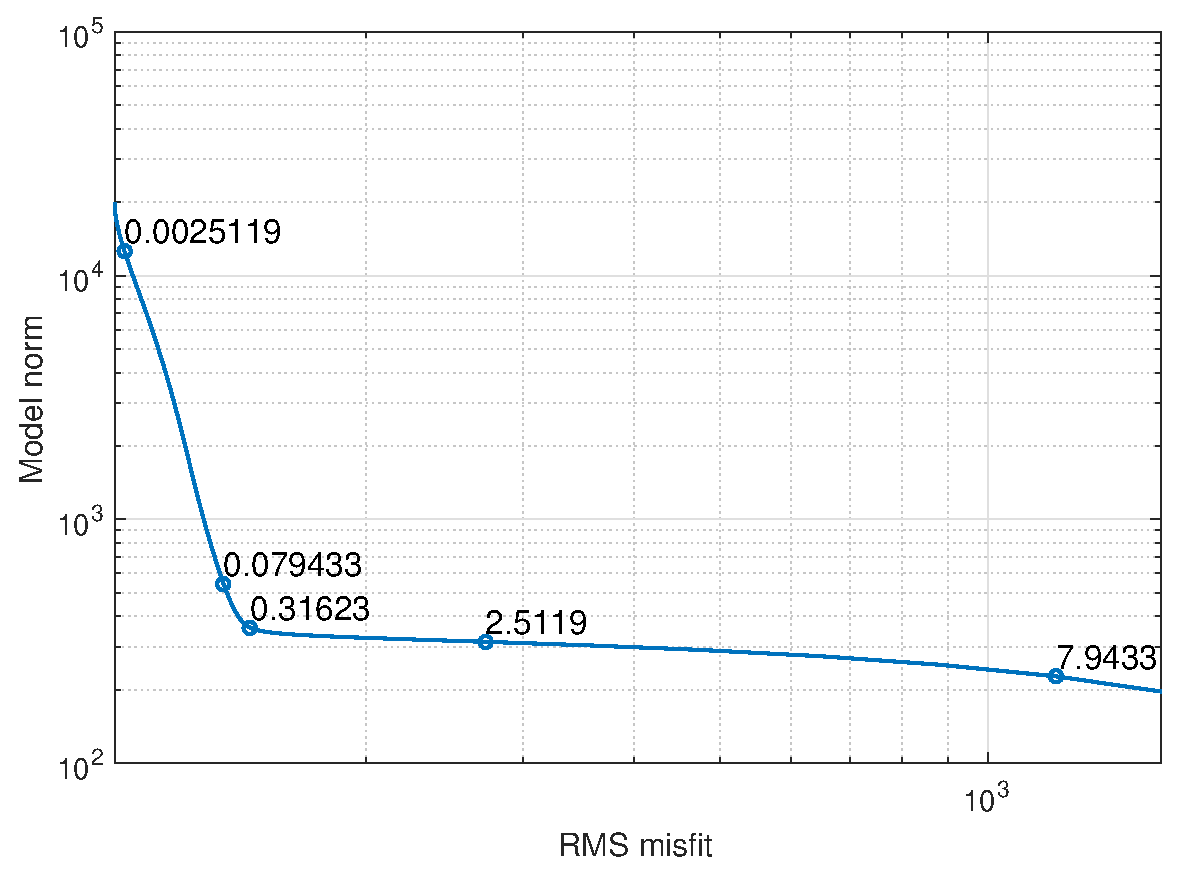
\includegraphics[width=\textwidth]{fig/LCurveBz.eps}
        \caption{Model based on $B_z$.}
        \label{fig:LCurveBz}
    \end{subfigure}
    
    ~ %add desired spacing between images, e. g. ~, \quad, \qquad, \hfill etc. 
      %(or a blank line to force the subfigure onto a new line)
    \begin{subfigure}[b]{0.45\textwidth}
        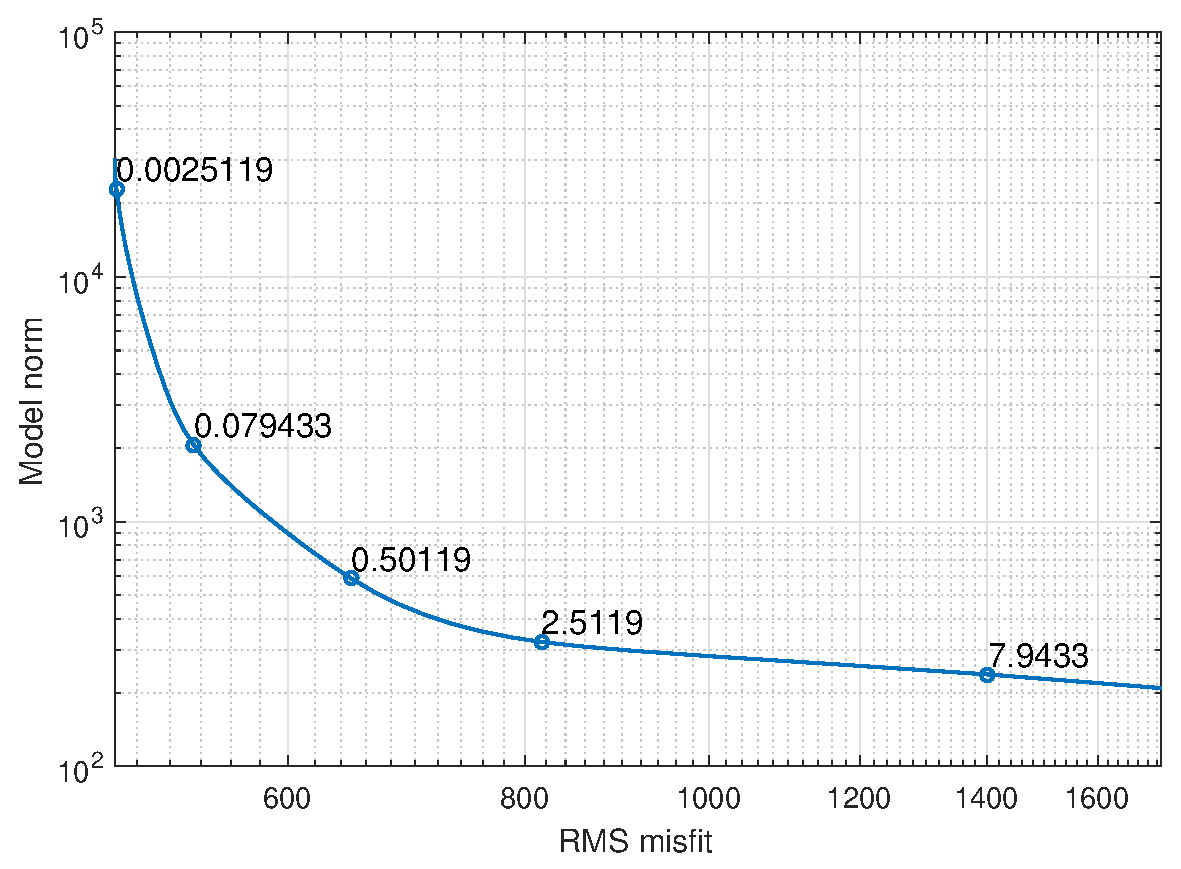
\includegraphics[width=\textwidth]{fig/LCurveBx.eps}
        \caption{Model based on $B_x$.}
        \label{fig:LCurveBx}
    \end{subfigure}
    ~ %add desired spacing between images, e. g. ~, \quad, \qquad, \hfill etc. 
    %(or a blank line to force the subfigure onto a new line)
    \begin{subfigure}[b]{0.45\textwidth}
        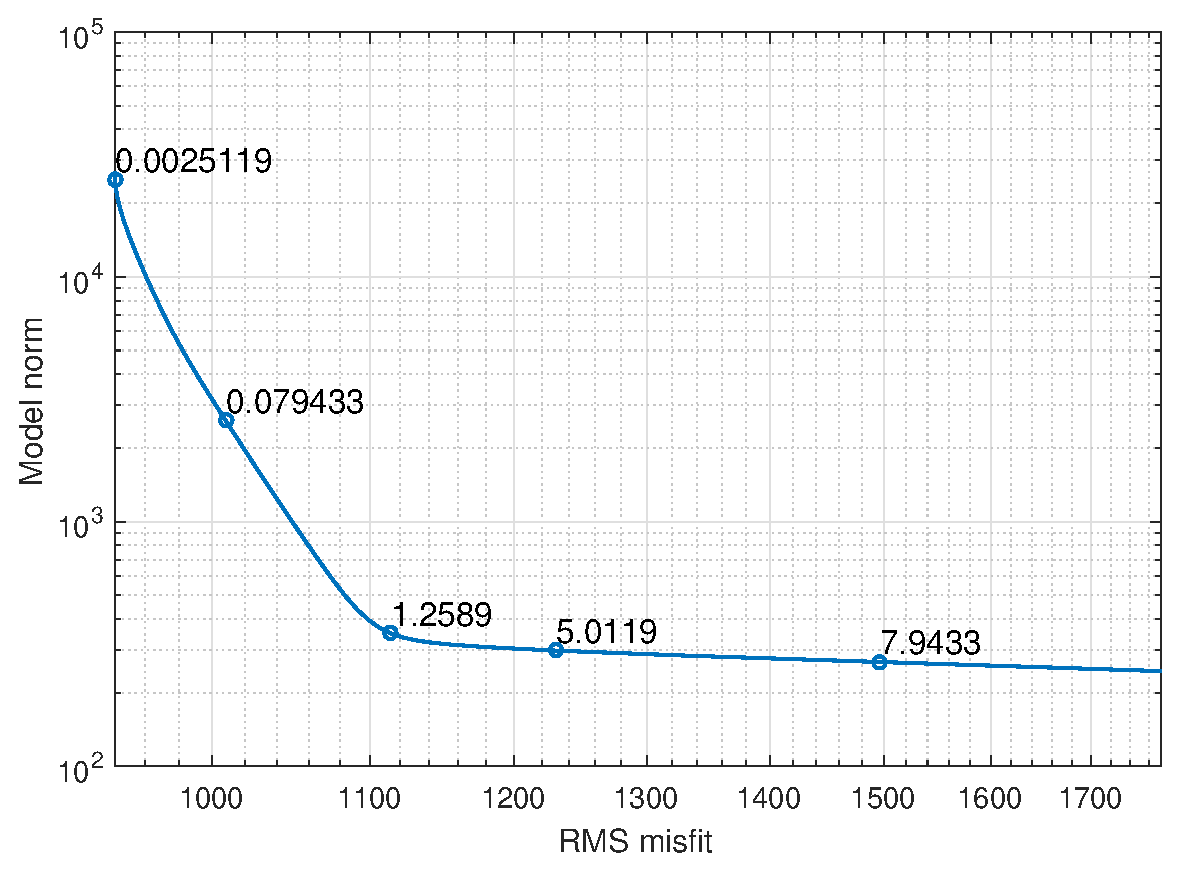
\includegraphics[width=\textwidth]{fig/LCurveBj.eps}
        \caption{Joint model}
        \label{fig:LCurveBj}
    \end{subfigure}
    \caption{L-curves with included alpha values.}
    \label{fig:LCurve}
\end{figure}

\begin{figure}[ht]
    \centering
    \begin{subfigure}[b]{0.45\textwidth}
        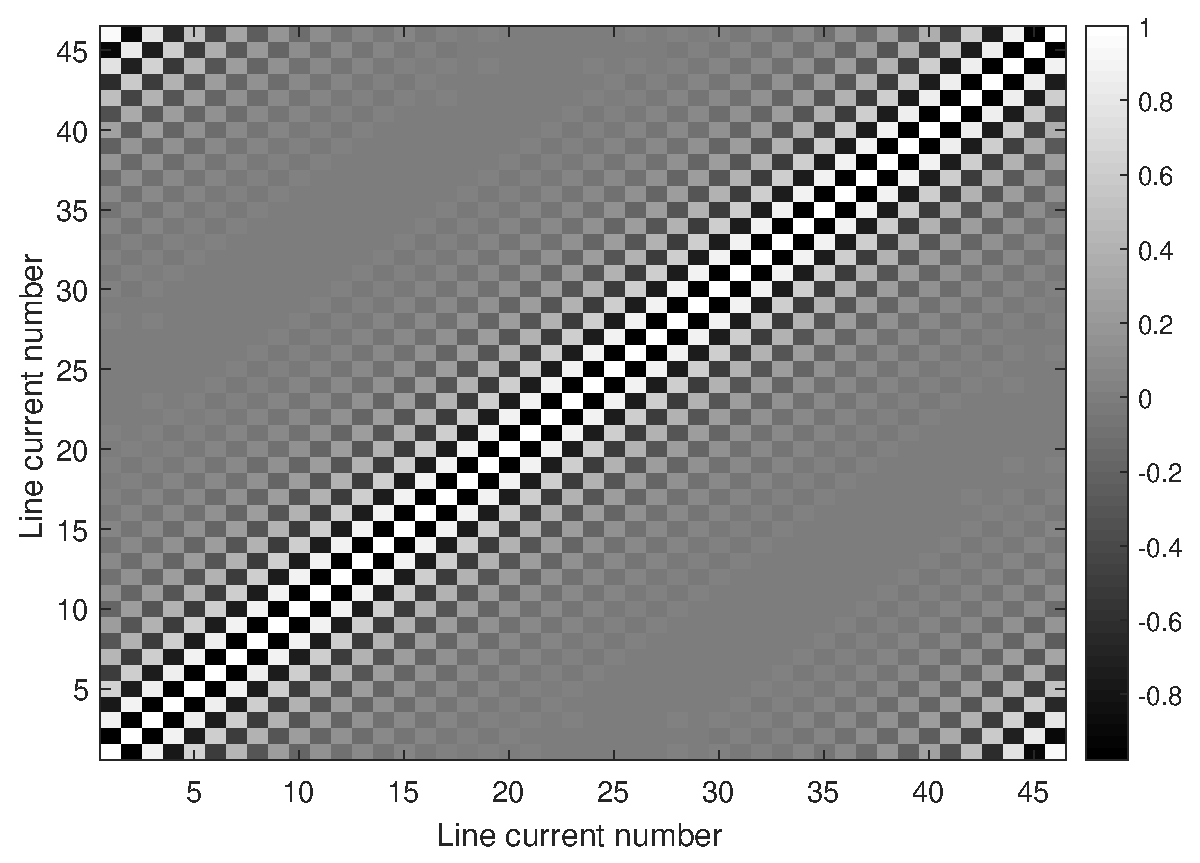
\includegraphics[width=\textwidth]{fig/corZ.eps}
        \caption{Model based on $B_z$.}
        \label{fig:corZ}
    \end{subfigure}
    
    ~ %add desired spacing between images, e. g. ~, \quad, \qquad, \hfill etc. 
      %(or a blank line to force the subfigure onto a new line)
    \begin{subfigure}[b]{0.45\textwidth}
        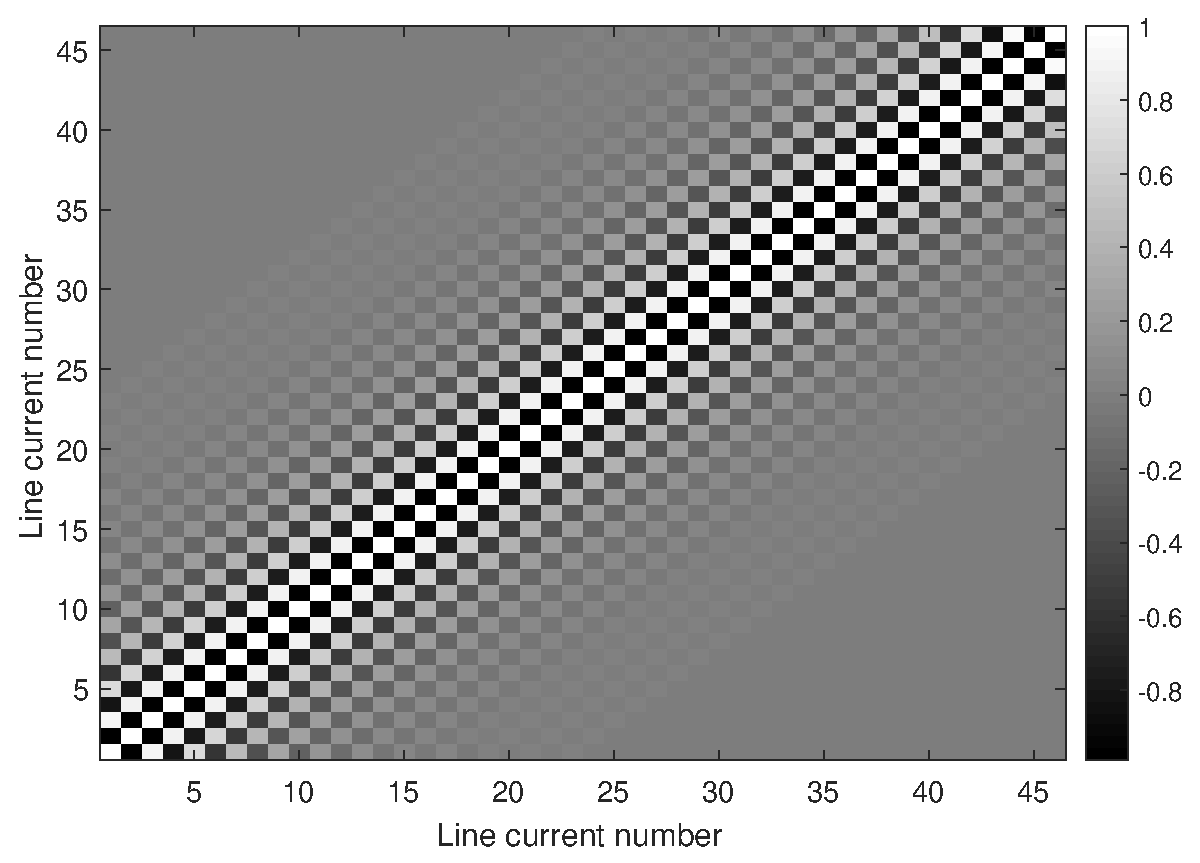
\includegraphics[width=\textwidth]{fig/corX.eps}
        \caption{Model based on $B_x$.}
        \label{fig:corX}
    \end{subfigure}
    ~ %add desired spacing between images, e. g. ~, \quad, \qquad, \hfill etc. 
    %(or a blank line to force the subfigure onto a new line)
    \begin{subfigure}[b]{0.45\textwidth}
        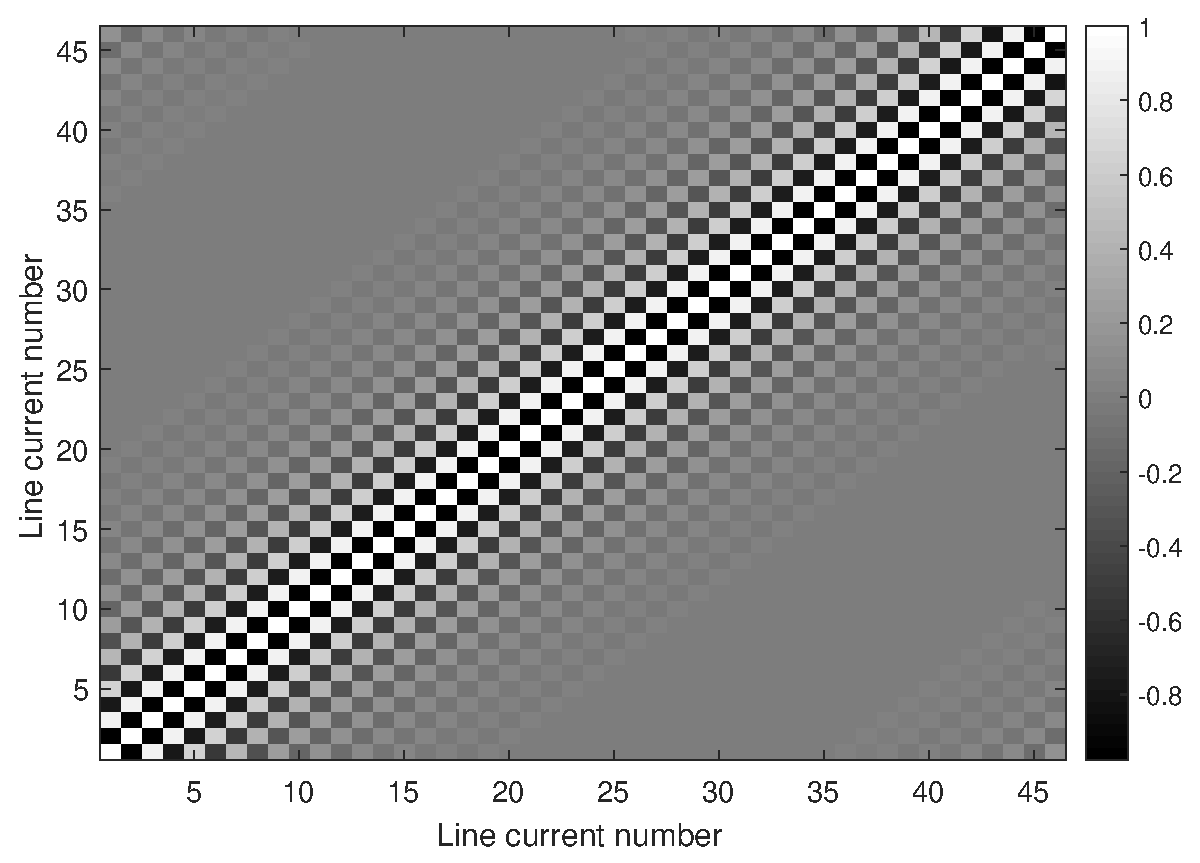
\includegraphics[width=\textwidth]{fig/corJ.eps}
        \caption{Joint model.}
        \label{fig:corJ}
    \end{subfigure}
    \caption{Correlation of chosen line currents.}
    \label{fig:cor}
\end{figure}

\begin{figure}[ht]
    \centering
    \begin{subfigure}[b]{0.45\textwidth}
        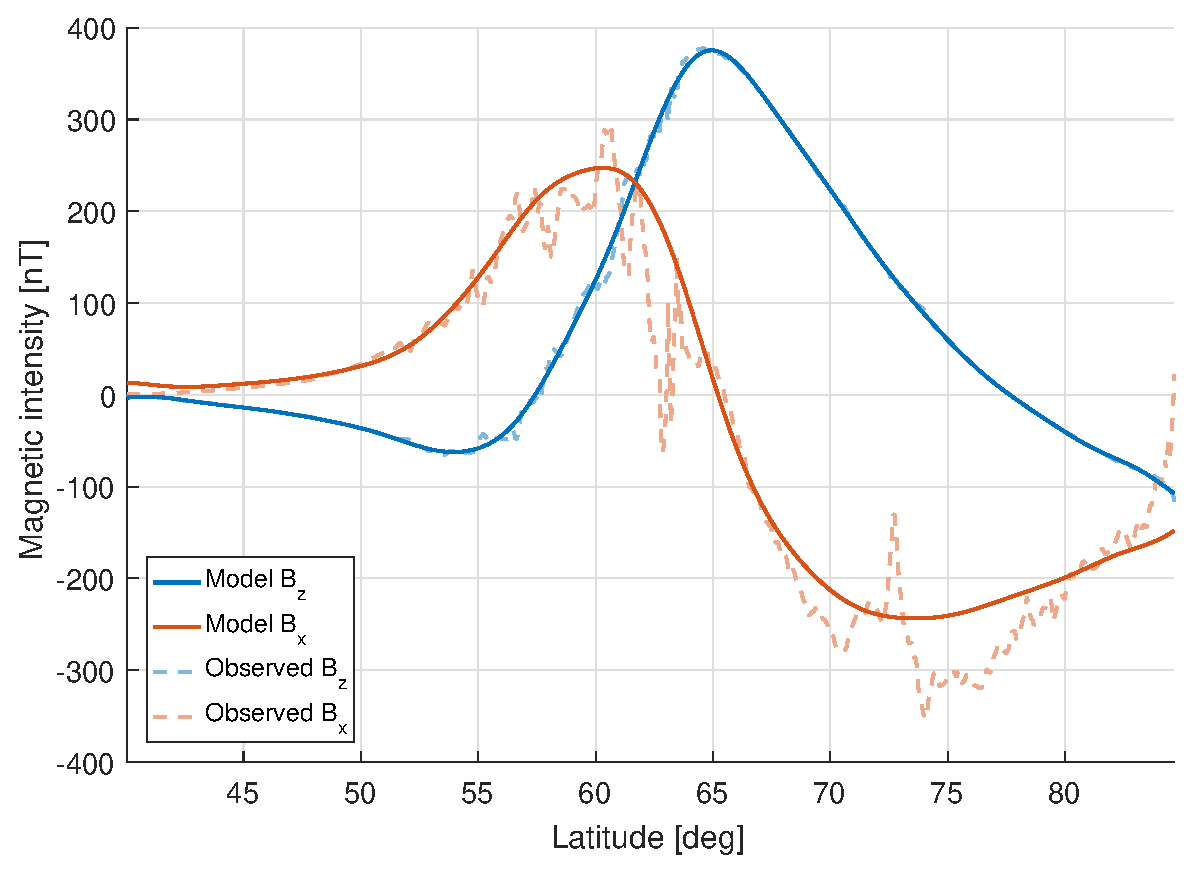
\includegraphics[width=\textwidth]{fig/BzModel.eps}
        \caption{Model based on $B_z$.}
        \label{fig:BzModel}
    \end{subfigure}
    
    ~ %add desired spacing between images, e. g. ~, \quad, \qquad, \hfill etc. 
      %(or a blank line to force the subfigure onto a new line)
    \begin{subfigure}[b]{0.45\textwidth}
        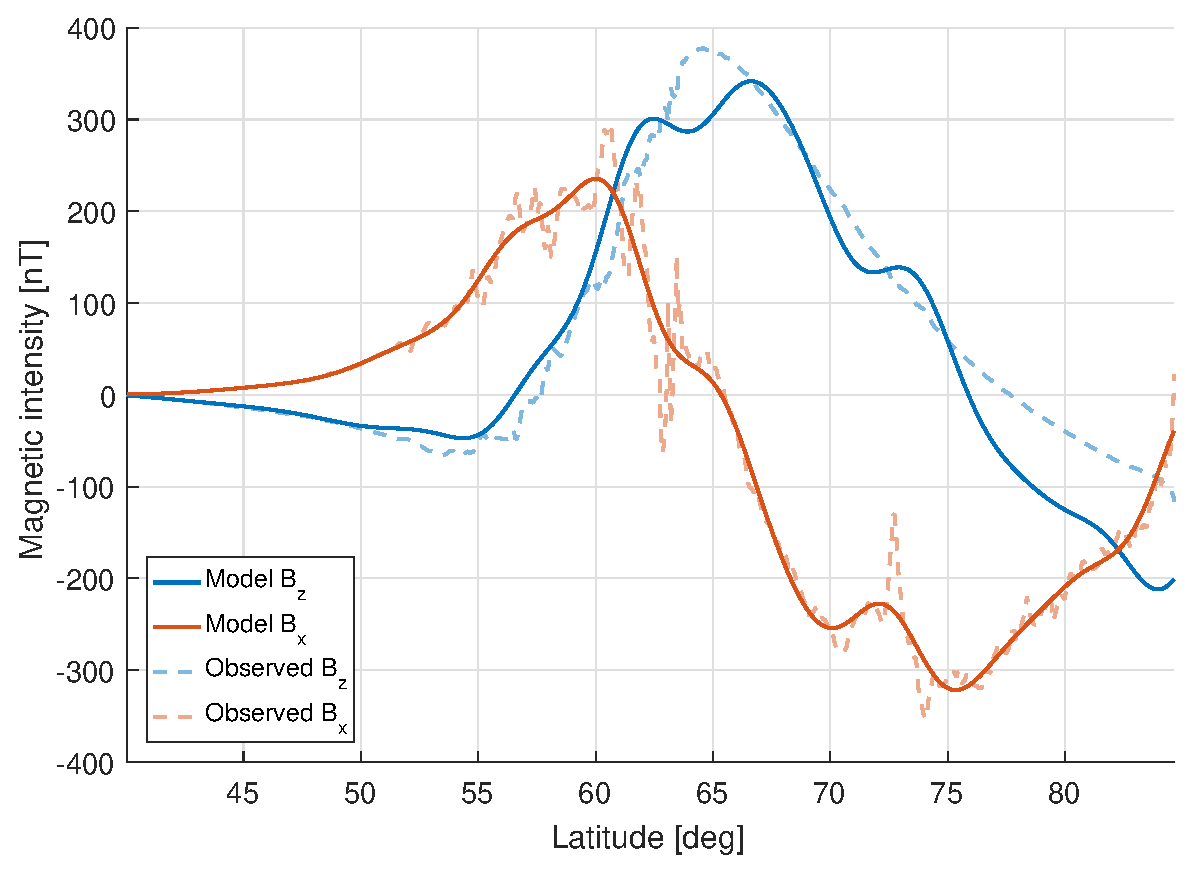
\includegraphics[width=\textwidth]{fig/BxModel.eps}
        \caption{Model based on $B_x$.}
        \label{fig:BxModel}
    \end{subfigure}
    ~ %add desired spacing between images, e. g. ~, \quad, \qquad, \hfill etc. 
    %(or a blank line to force the subfigure onto a new line)
    \begin{subfigure}[b]{0.45\textwidth}
        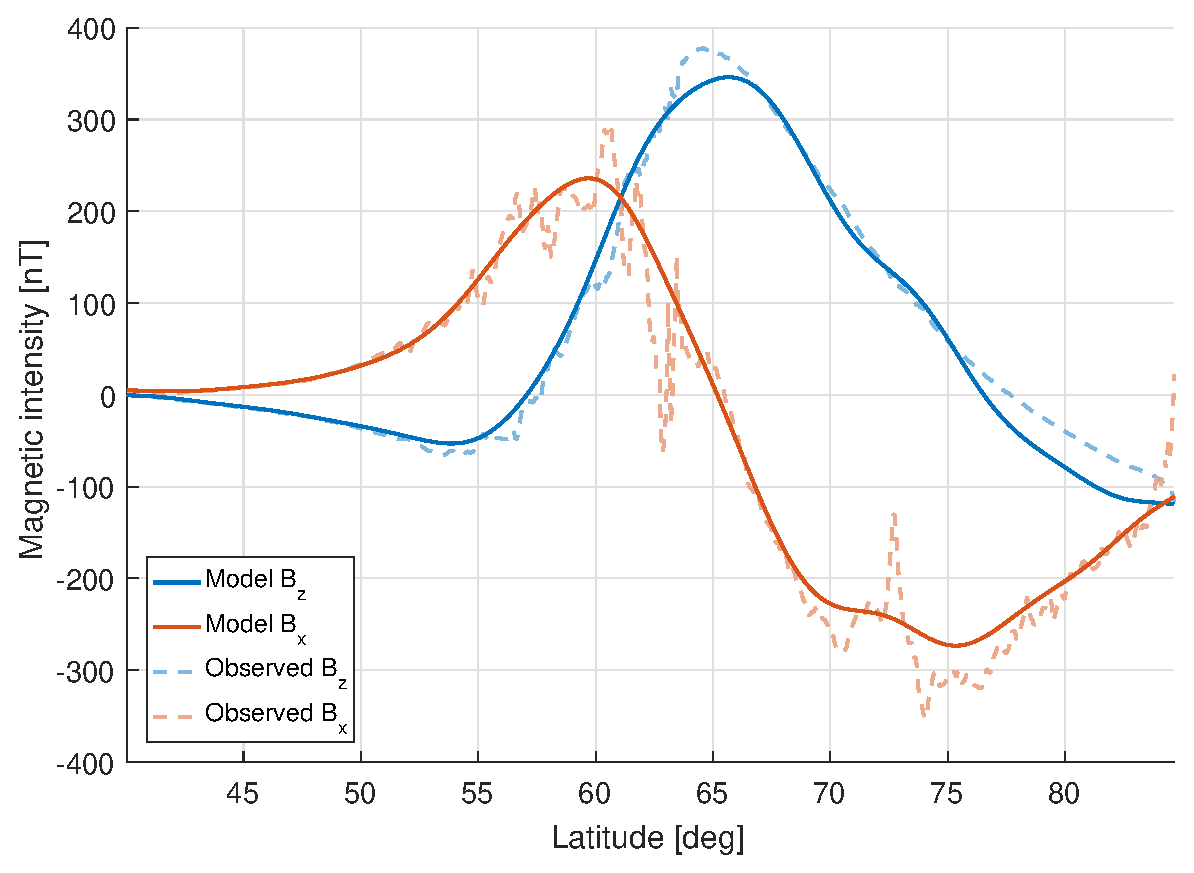
\includegraphics[width=\textwidth]{fig/BjModel.eps}
        \caption{Joint model}
        \label{fig:BjModel}
    \end{subfigure}
    \caption{Modeled magnetic field in $z$ and $x$ direction. Includes both the modeled data as well as the opbserved data.}
    \label{fig:model}
\end{figure}

\begin{figure}[ht]
    \centering
    \begin{subfigure}[b]{0.45\textwidth}
        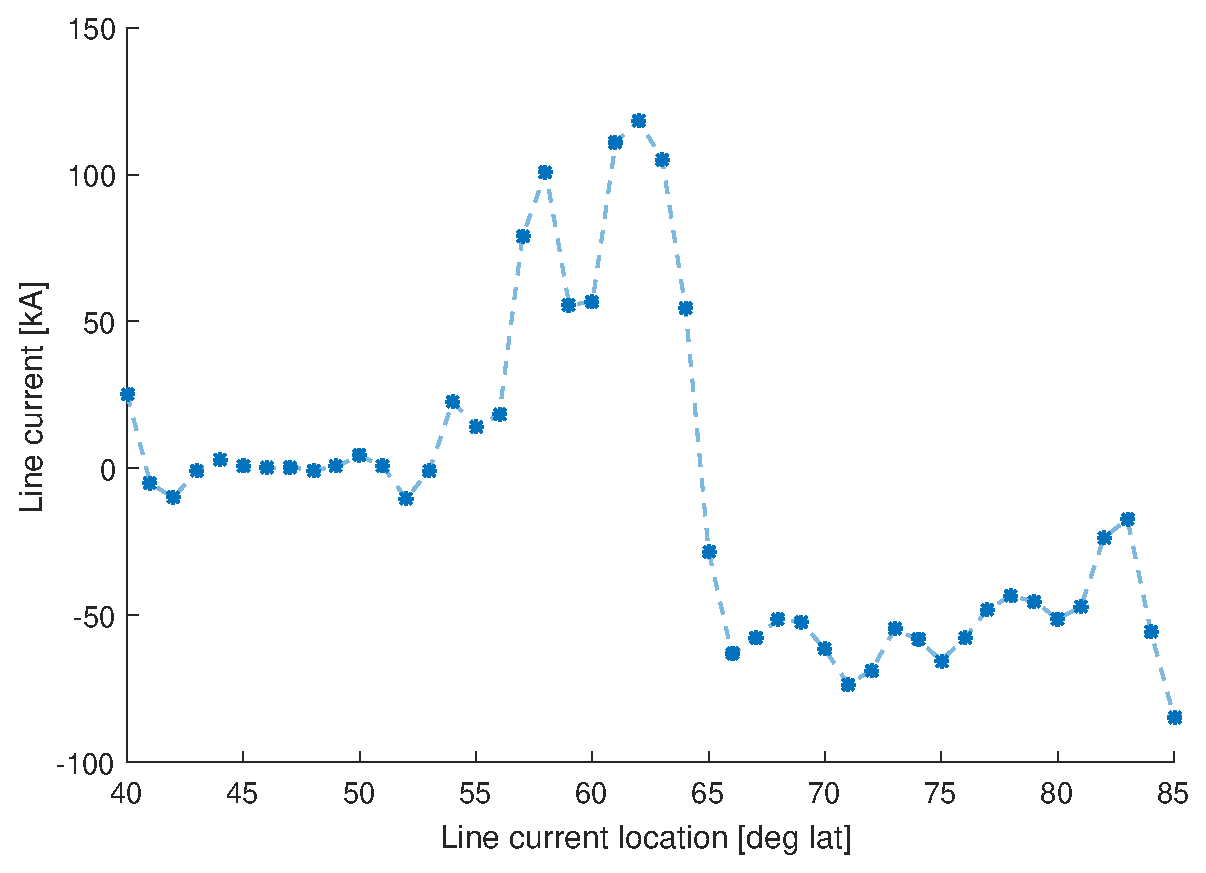
\includegraphics[width=\textwidth]{fig/LCz.eps}
        \caption{Model based on $B_z$.}
        \label{fig:LCz}
    \end{subfigure}
    
    ~ %add desired spacing between images, e. g. ~, \quad, \qquad, \hfill etc. 
      %(or a blank line to force the subfigure onto a new line)
    \begin{subfigure}[b]{0.45\textwidth}
        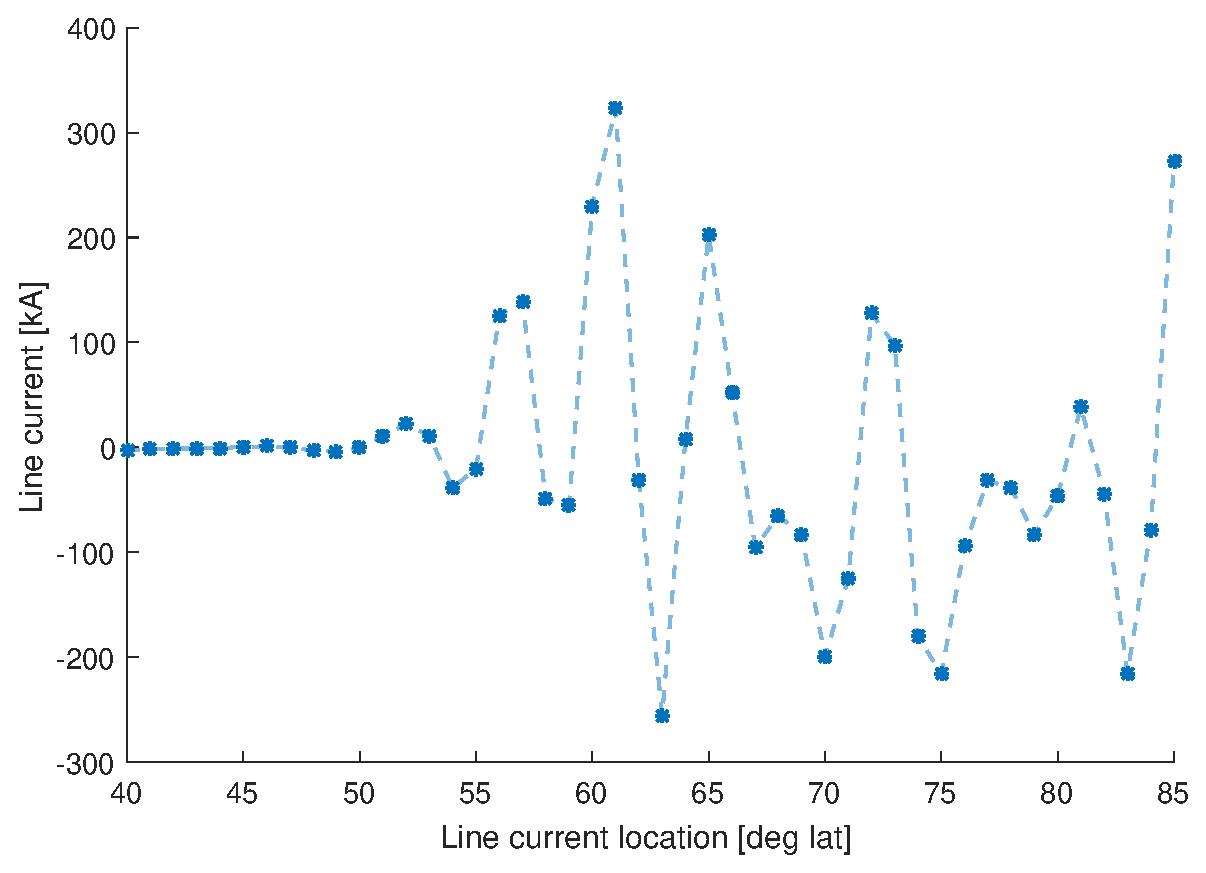
\includegraphics[width=\textwidth]{fig/LCx.eps}
        \caption{Model based on $B_x$.}
        \label{fig:LCx}
    \end{subfigure}
    ~ %add desired spacing between images, e. g. ~, \quad, \qquad, \hfill etc. 
    %(or a blank line to force the subfigure onto a new line)
    \begin{subfigure}[b]{0.45\textwidth}
        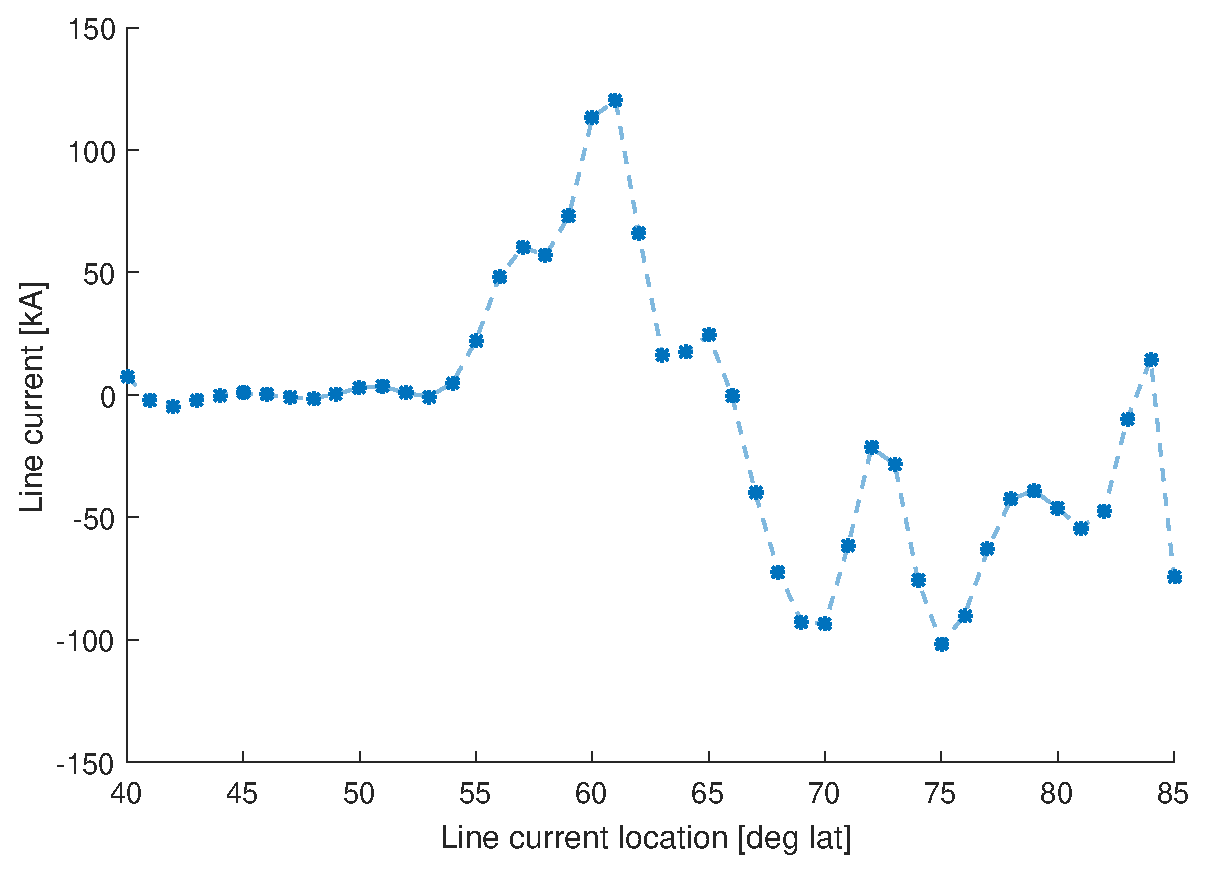
\includegraphics[width=\textwidth]{fig/LCj.eps}
        \caption{Joint model}
        \label{fig:LCj}
    \end{subfigure}
    \caption{Modeled line currents. The line indicates the continuous current, and the markers the discrete line currents.}
    \label{fig:LC}
\end{figure}